\parindent=0em
\subsection{Pruebas}
\noindent

Para poder obtener una serie de conclusiones acertadas, en primer lugar se han definido tres pruebas distintas. \\

En el primer escenario que se tendrá en cuenta se resumen todas las variables a considerar (Forma de los puntos, máximo numero de puntos y máximo número de puntos a añadir por \textit{frame}). Con ello se obtendrá la media de rendimiento de cada una de estas situaciones. Encontramos 5 tipos distintos de formas a considerar (Esfera, Cubo, Quad, Cilindro y Cápsula). Con cada una de estas formas se generarán pruebas combinando los distintos valores del máximo de puntos posibles (1000, 10000 y 20000) y el número máximo de puntos que podemos añadir por cada \textit{frame} (1, 10 o 100). Estos valores, tanto para el número máximo de puntos como para el máximo de puntos añadidos por \textit{frame}, no son aleatorios. \\

En el caso del máximo número de puntos posibles, 1000 es un valor que permanece neutro mientras que 20.000 es un valor demasiado alto que en muy pocas circunstancias se llega a alcanzar. En lo referente al máximo número de puntos por \textit{frame}, se ha de tener en cuenta que el número aquí introducido influirá directamente en el tiempo que tarde en realizarse el bucle principal de la aplicación. A partir de 100 la aplicación tiene un rendimiento totalmente nulo y 1 es el valor por defecto y el mínimo que se puede aplicar. Esto deja un total de 45 pruebas a realizar por cada una de las perspectivas que se quieran tener en cuenta.\\

Una vez estén todos estos datos encapsulados, se procede a realizar la media de rendimiento por cada una de las formas que hemos utilizado. Así encontramos una primera aproximación a los datos que queremos analizaremos más adelante.\\

\begin{table}[ht]
\centering
\resizebox{0.6\textwidth}{!}{
\begin{tabular}{cc}
\toprule
Forma & Media de rendimiento (FPS) \\ \toprule
\textit{Esfera }       & 17.88   \\ \midrule
\textit{Cubo}      & 15.72          \\ \midrule
\textit{Quad}       & 15.27         \\ \midrule
\textit{Cilindro}         & 11.33          \\ \midrule
\textit{Cápsula} & 9.55   \\ \bottomrule
\end{tabular}}
\caption{Media de \textit{Frames} Por Segundo (FPS) para cada una de las formas disponibles a la hora de realizar la oclusión. }
\label{cuadro:mediaRendimiento}
\end{table}

Con esta primera aproximación en la que se puede ver lo que ha costado todo el proceso, desde la generación de la nube de puntos hasta el renderizado de la misma,  fácilmente se aprecia que la forma con la que se obtiene mejor rendimiento (de media) es la esfera.\\

Este rendimiento está influido por la forma de la figura ya que en esta varía el número de polígonos a la hora de ser renderizada, por lo que el resultado final sólo es orientativo para proseguir con las pruebas. \\

Sabiendo que la esfera es de promedio la forma con mejores resultados, se utilizará para realizar la siguiente prueba. Esta consiste en probar únicamente el tiempo en el que una nube de puntos tarda en estabilizarse. Para ello, se tendrá en cuenta el instante en el que comenzamos la prueba y el instante en el que la nube de puntos ha alcanzado su estabilidad. \\

Esta estabilidad se da por asumida cuando se han generado el máximo número de puntos establecido. Se realizará únicamente con las medidas de máximo de puntos que se pueden añadir a la escena y con el máximo de puntos que se pueden añadir por \textit{frame}. Las mediciones se llevarán a cabo dos veces para obtener la media de ambas pruebas y poder tener en cuenta otros factores como la iluminación del entorno o el número de objetos que en él se encuentren.\\

\begin{table}[H]
\centering
\resizebox{0.55\textwidth}{!}{
\begin{tabular}{ccc}
\toprule
Máx. Puntos & Puntos por \textit{frame} & Media de tiempo (s)\\ \toprule
 1.000 & 1 & 15.03   \\ \midrule
1.000 & 10 & 7.75  \\ \midrule
1.000 & 100 & 5.97  \\ \midrule
10.000  & 1 & 18.98 \\ \midrule
10.000  & 10 & 11.63 \\ \midrule
10.000  & 100 & 7.84 \\ \midrule
20.000  & 1 & 22.21 \\ \midrule
20.000  & 10 & 16.19 \\ \midrule
20.000 & 100 & 11.31  \\ \bottomrule
\end{tabular}}
\caption{Tiempo empleado por la aplicación para generar una nube de puntos estable. }
\label{cuadro:comparacionpesopreciosHMD}
\end{table}

Realizada esta prueba se puede apreciar que la combinación que toma menos tiempo para realizar la nube de puntos es la que cuenta con un número máximo de 1.000 puntos y un número de 100 puntos por \textit{frame}. Esta medida era lógica y esperada, ya que 1.000 es el número menor de puntos y que generando 100 puntos por \textit{frame} tenemos un crecimiento bastante rápido de la nube. Evidentemente esta última medida afecta notoriamente al rendimiento de la aplicación. Este resultado en el futuro nos ayudará a decidir cual es la mejor manera de generar la oclusión dentro de la aplicación.\\

La última prueba a realizar consistirá en unir todas las formas mencionadas y distintos tamaños para la oclusión. Para ello utilizaremos la prueba \textit{Test Visualization} de la aplicación explicada en profundidad en el apartado anterior.\\

Finalmente, todas estas imágenes se procesarán con la aplicación escrita en Python tal y como se explicó en el apartado anterior.\\

\begin{figure}[H]
    \centering
    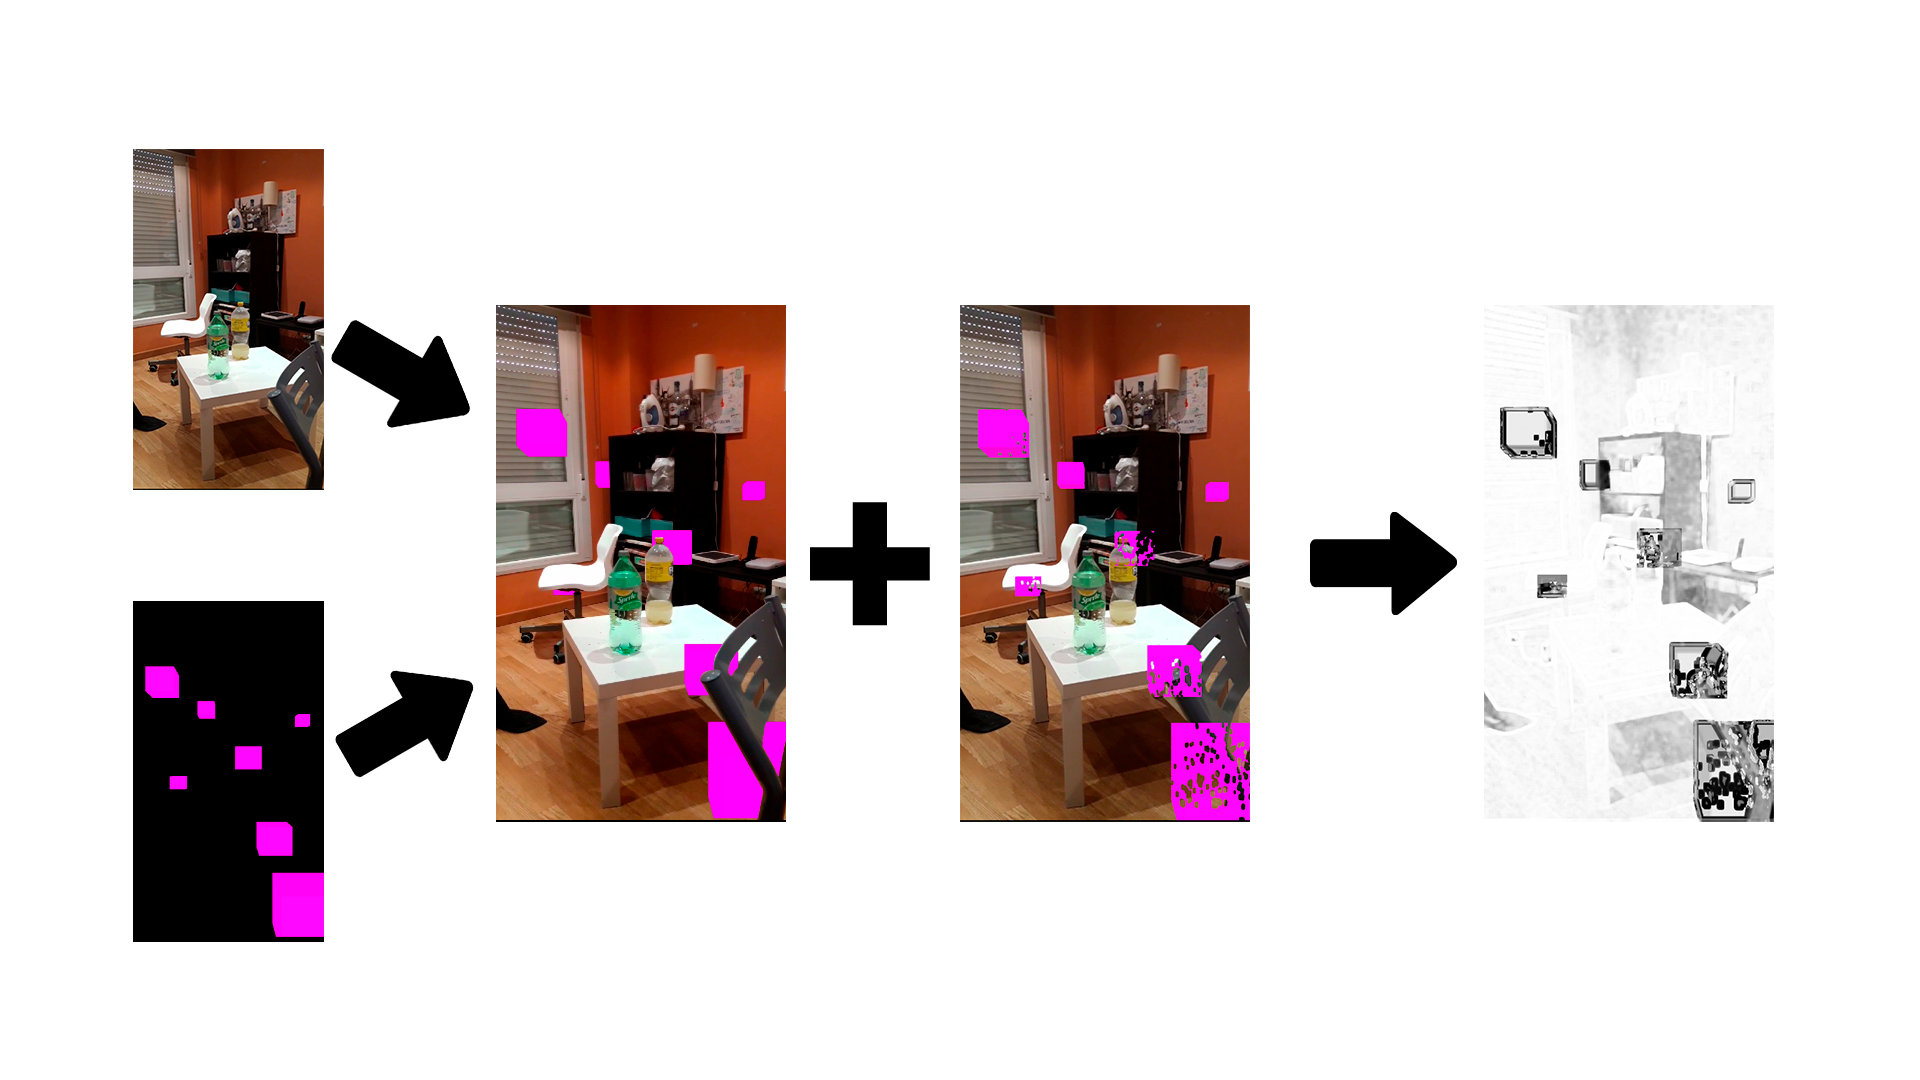
\includegraphics[scale=0.2]{Images/NubeDePuntos/ComparacionImagenes.png}
    \caption[\textit{Workflow} de comparación de imágenes.]{\textit{Workflow} de comparación de imágenes.}
    \label{fig:AppUnity}
    \end{figure}

En la siguiente tabla mostramos cual ha sido el mejor tamaño para cada una de las formas en base a su acierto medio.\\

\begin{table}[ht]
\centering
\resizebox{0.4\textwidth}{!}{
\begin{tabular}{ccc}
\toprule
Forma & Tamaño & Acierto \\ \toprule
Esfera & 0.05 & 85,92\%   \\ \midrule
Cubo & 0.04 & 85,79\%   \\ \midrule
Quad & 0.04 & 86,85\%   \\ \midrule
Cilindro & 0.01 & 86.65\%   \\ \midrule
Cápsula & 0.05 & 88.22\%  \\ \bottomrule
\end{tabular}}
\caption{Distintas formas para general la oclusión y tamaños con sus correspondientes porcentajes de acierto. }
\label{cuadro:javicabronque has copiado la referencia y no me iba}
\end{table}

Este resultado indica que la forma \textit{Cápsula}, con tamaño 0,05 es la que mejor porcentaje de acierto tiene de entre todas las pruebas realizadas. Sin embargo, si se observa el (cuadro \ref{cuadro:mediaRendimiento}), podemos apreciar que es la que peor rendimiento obtiene.\\

Si se buscase un termino medio que aunase el resultado de la oclusión, con el número de puntos generados y el tiempo que tardan en generarse estos, así como la media de rendimiento de la aplicación, basándonos en los tres cuadros anteriores podríamos apreciar que:

\begin{itemize}
         \item La esfera tiene una tasa de acierto media aceptable (85,92\%)
         \item La esfera tiene la mejor media de rendimiento (17.88 FPS)
         \item Una media razonable de puntos a añadir sería de 10.000 puntos con 10 puntos añadidos por \textit{frame}, ya que tiene un valor intermedio en tiempo de creación (11.63 s) y no afecta extraordinariamente al rendimiento.
\end{itemize}